\documentclass[tikz,border=20pt]{standalone}

\usepackage{amsmath}
\usepackage{amsfonts}
\usetikzlibrary{positioning}

\begin{document}
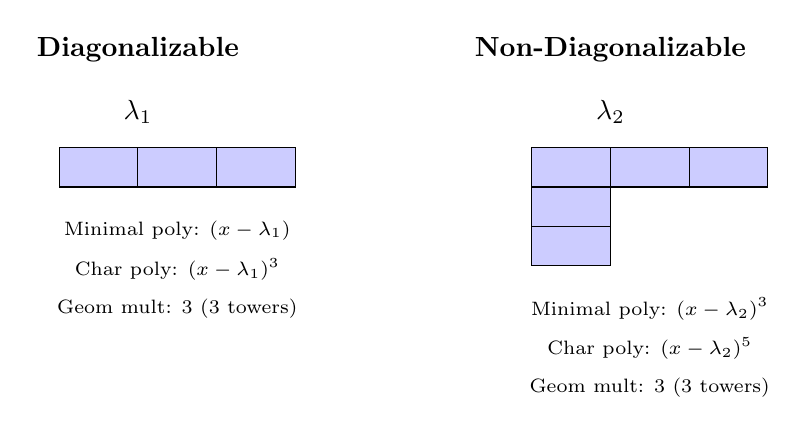
\begin{tikzpicture}[block/.style={draw, fill=blue!20, minimum width=1cm, minimum height=0.5cm}]

    % Titles
    \node at (0,4.5) {\textbf{Diagonalizable}};
    \node at (6,4.5) {\textbf{Non-Diagonalizable}};

    % Diagonalizable eigenvalue (lambda_1)
    \node at (0,3.7) {$\lambda_1$};

    % Towers for diagonalizable case: 3 blocks, size 1 each
    \node[block] (d1a) at (-0.5,3) {};
    \node[block] (d1b) at (0.5,3) {};
    \node[block] (d1c) at (1.5,3) {};

    % Label for diagonalizable minimal polynomial
    \node at (0.5,2.2) {\scriptsize Minimal poly: $(x-\lambda_1)$};

    % Algebraic multiplicity note
    \node at (0.5,1.7) {\scriptsize Char poly: $(x-\lambda_1)^3$};

    % Geometric multiplicity note
    \node at (0.5,1.2) {\scriptsize Geom mult: $3$ (3 towers)};

    % Non-diagonalizable eigenvalue (lambda_2)
    \node at (6,3.7) {$\lambda_2$};

    % Towers for non-diagonalizable case: blocks of size 3, 1, 1
    \node[block] (nd1a) at (5.5,3) {};
    \node[block] (nd1b) at (5.5,2.5) {};
    \node[block] (nd1c) at (5.5,2.0) {};

    \node[block] (nd2a) at (6.5,3) {};
    \node[block] (nd3a) at (7.5,3) {};

    % Labels for non-diagonalizable minimal poly
    \node at (6.5,1.2) {\scriptsize Minimal poly: $(x-\lambda_2)^3$};

    % Char poly note
    \node at (6.5,0.7) {\scriptsize Char poly: $(x-\lambda_2)^5$};

    % Geometric multiplicity note
    \node at (6.5,0.2) {\scriptsize Geom mult: $3$ (3 towers)};

\end{tikzpicture}

\[
    \footnotesize
    \begin{aligned}
         &
        \Lambda_{\text{diag}} =
        \begin{bmatrix}
            \lambda_1 & 0         & 0         \\
            0         & \lambda_1 & 0         \\
            0         & 0         & \lambda_1
        \end{bmatrix}
        \qquad
         &
        \Lambda_{\text{non-diag}} =
        \begin{bmatrix}
            \lambda_2 & 0         & 0         & 0         & 0         \\
            0         & \lambda_2 & 0         & 0         & 0         \\
            0         & 0         & \lambda_2 & 1         & 0         \\
            0         & 0         & 0         & \lambda_2 & 1         \\
            0         & 0         & 0         & 0         & \lambda_2 \\
        \end{bmatrix}
        \\[1em]
         &
        \text{\small Jordan blocks: }
         &
        \text{\small Jordan blocks: }
        \\
         &
        \begin{bmatrix}
            \lambda_1
        \end{bmatrix}
        \! , \;
        \begin{bmatrix}
            \lambda_1
        \end{bmatrix}
        \! , \;
        \begin{bmatrix}
            \lambda_1
        \end{bmatrix}
         &
        \begin{bmatrix}
            \lambda_2
        \end{bmatrix}
        \! , \;
        \begin{bmatrix}
            \lambda_2
        \end{bmatrix}
        \! , \;
        \begin{bmatrix}
            \lambda_2 & 1         & 0         \\
            0         & \lambda_2 & 1         \\
            0         & 0         & \lambda_2
        \end{bmatrix}
    \end{aligned}
\]
\[
    \begin{aligned}
         & \footnotesize \text{Generalized eigenspace for } \lambda_j: \\
         & G_{\lambda_j} = \ker ( (T - \lambda_j I)^{k_j} ),
        \quad
        V = \bigoplus_{j=1}^s G_{\lambda_j}
    \end{aligned}
\]

\pagebreak

\small

\textbf{Theorem (Primary Decomposition).}
Let $T \colon V \to V$ be a linear operator on a finite-dimensional vector space $V$ over $\mathbb{C}$, and let
\[
    m_T(x) = \prod_{j=1}^s (x - \lambda_j)^{k_j}
\]
be the factorization of the minimal polynomial of $T$ into powers of distinct linear factors. Then
\[
    V = \bigoplus_{j=1}^s V_j,
    \qquad \text{where }
    V_j = \ker\!\big( (T - \lambda_j I)^{k_j} \big).
\]
Each $V_j$ is $T$-invariant, and the restriction $T|_{V_j}$ has minimal polynomial $(x - \lambda_j)^{k_j}$.


\end{document}
